\section{Pattern recognition and track fitting approaches}

\subsection{Introduction to associative memory approach}

\noindent The SVT approach at CDF was the first hadron collider experiment in HEP to incorporate a fast secondary vertex track trigger~\cite{bib:Ade-06}, \cite{bib:Ade-07} to find all tracks produced in each collision and precisely measure their properties within about 30 microseconds from the time of the collision. The SVT significantly extended the physics reach of CDF opening the way to measurements that would have been impossible otherwise.

\noindent The CDF SVT-style associative memory approach, later adopted for FTK, consists of two sequential steps of increasing resolution.  In step 1, pattern recognition is carried out by a dedicated device called the Associative Memory (AM) which finds track candidates in coarse resolution roads.  When a road has stubs on all layers or all except one, step 2 is carried out in which the full resolution hits within the road are fit to determine the track helix parameters and a goodness of fit.  Tracks that pass a  2 cut are kept.  If there are hits in all layers and the  2 fails the cut but is not extremely large, the track is refit a number of times with the hit on one of the layers dropped each time.  This "majority recovery" allows for the loss of a single hit/stub due to detector inefficiency with a random hit picked up instead. 

\noindent Note that there has been more than a decade of experience in HEP with this approach from both CDF and Atlas, though all with silicon-based tracking trigger for Level 2 where trigger latency requirement is much more relaxed.  Therefore, one of the key issues for L1 implementation or demonstration will be the overall tracking trigger latency. Both the pattern recognition at the AM stage (hits delivery) and track fitting stage will have to be fast enough.


\subsubsection{From pattern recognition to track fitting}

\noindent The pattern recognition step is usually the most time consuming task, because one needs to test many combinations of hits to find those that potentially come from the same track and typically these tests are done sequentially (e.g. in software). The associative memory approach allows the testing of all hit combinations in parallel against a set of known patterns. To illustrate the concept of patterns in the associative memory approach, one can use an oversimplified case with a simple detector consisting of six detector layers, as shown in Fig.~\ref{fig:AM_principle_1}. A charged track crossing the detector would produce a set of hits (pattern). A finite set of distinct patterns can be generated this way using valid tracks for a given experiment, and such sets are often called the pattern bank. 

\begin{figure}[ht!]
\centering
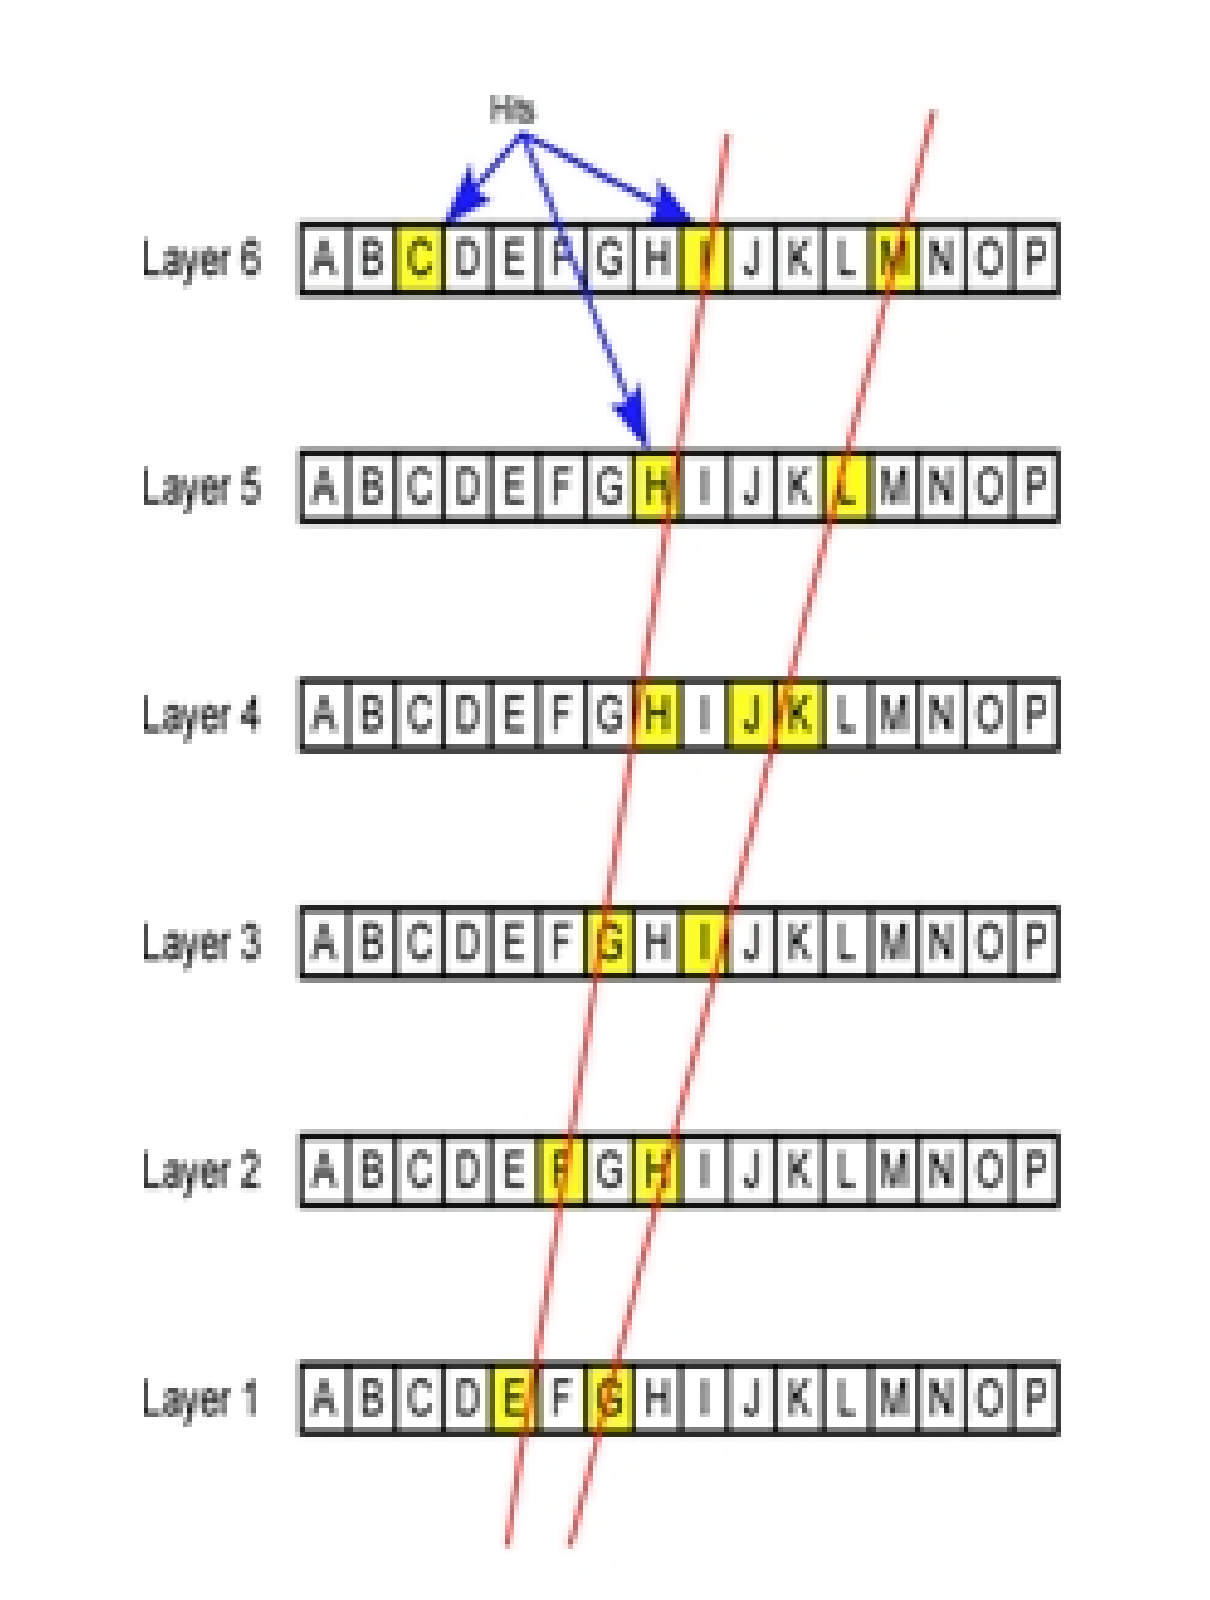
\includegraphics[width=0.4\columnwidth]{Plots/AM_pple2.eps}
\caption{Tracks in a tracking detector}
\label{fig:AM_principle_1}
\end{figure}

\noindent The Associative Memory (AM) architecture is based on Content Addressable Memory (CAM) cells~\cite{bib:Koh-87,bib:Pag-06} to efficiently identify track patterns (roads) at high speed using coarse-resolution 'hits' recorded in the tracking detector. A block diagram~\cite{bib:Rist-89} of the Associative Memory architecture is shown in Fig. 2 (for a case with four detector layers).  Each pattern (shown as a cell) is composed of four hit coordinates each of which is stored in the CAM word for a given layer, and only four patterns (cell 0 to 3) are shown in Fig.~\ref{fig:AM_principle_2}. 

\begin{figure}[ht!]
\centering
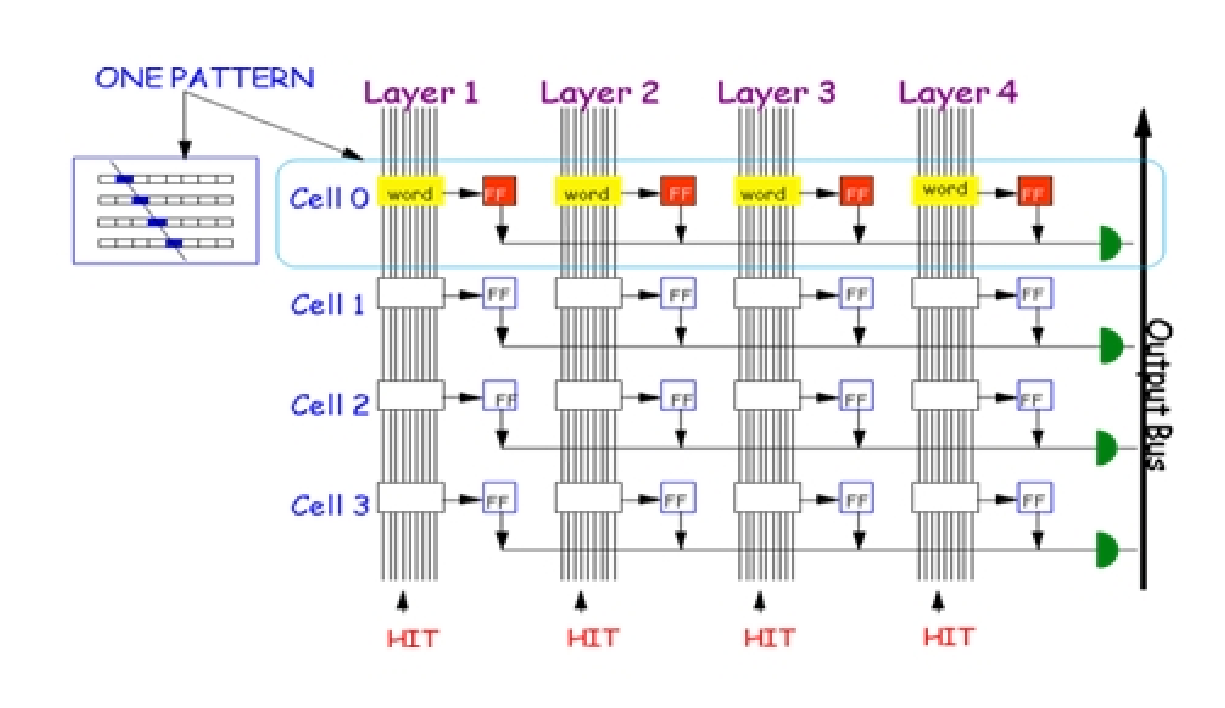
\includegraphics[width=0.9\columnwidth]{Plots/AM_pple.eps}
\caption{A block diagram on an associative memory chip. The CAM cells are shown as white (or yellow) boxes. The majority/glue logic is shown to the right as semi-circles.}
\label{fig:AM_principle_2}
\end{figure}

\noindent An incoming hit from a given detector layer is transmitted to the corresponding layer and the hit coordinate is compared against the stored words for all patterns in parallel for that layer. Any match to each incoming hit will be latched for that layer an
d for that pattern until reset (to rearm for next event). This process is repeated for all the incoming hits for each detector layer as the hits arrive one after the other. As soon as all hits from the same event are received, the hit matching stage is done and all latched matches for each pattern (or cell) will be fed into a majority logic stage where a fired road will be found if the number of matched layers reaches a programmable threshold. 
 

\noindent Associative Memory is sometimes called PRAM, Pattern Recognition Associative Memory. The AM method solves the combinatorial challenge inherent to the pattern recognition by exploiting massive parallelism of associative memories that can compare tracking detector hits to a set of pre-calculated patterns simultaneously. The found patterns or "fired roads" are then processed using fast FPGAs to perform track fitting with full detector resolution using all combinations of the "hits of interest" from the fired roads. Because each pattern or road is narrow enough, the usual helical fit can be replaced by a simple linear calculation. The track fitting stage for each matched pattern is much simplified and can be very fast~\cite{bib:Ann-09}.

\subsection{Trigger Tower, Sector, superstrip, and pattern banks}

\noindent We have described the concept of Trigger Tower in Section 2. Here we will describe the concept of sector, superstrip and pattern banks for the AM approach.

\noindent The pattern generation procedure starts by identifying first the sectors, which consists of one silicon module in each detector/logical layer. The list of sectors is determined with a training procedure that uses a large number of single muon (negative and positive) events, to cover all possible combinations of modules compatible with tracks coming from a region around the nominal beam spot position. The concept of sector is important because it is the region in which the linear track fit with one set of constants is performed (see later track fitting stage).

\noindent Each pattern is made of one superstrip per layer. A superstrip is a group of strips/pixels, and is therefore heavily constrained by the detector itself. Once the superstrip definition has been set, its position information is coded in a N-bits word: the superstrip address. It is important to realize that the AM-based pattern recognition is using these addresses, and is therefore independent from the detector geometry. As the addresses are transmitted to the AM independently for each layer, layer number doesn't have to be in the address word. 

\begin{figure}[ht!]
\centering
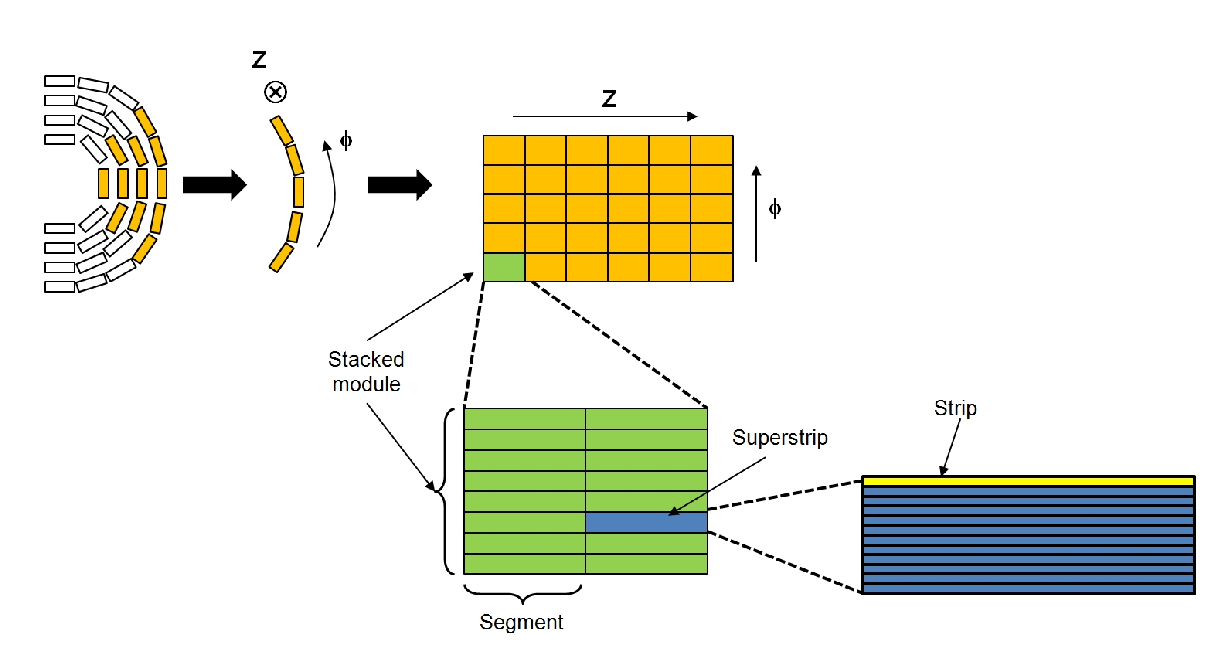
\includegraphics[width=0.8\columnwidth]{Plots/SStripDef.eps}
\caption{Geometric definition of a superstrip (barrel example).}
\label{fig:Det_to_SS}
\end{figure}
\begin{figure}[ht!]
\centering
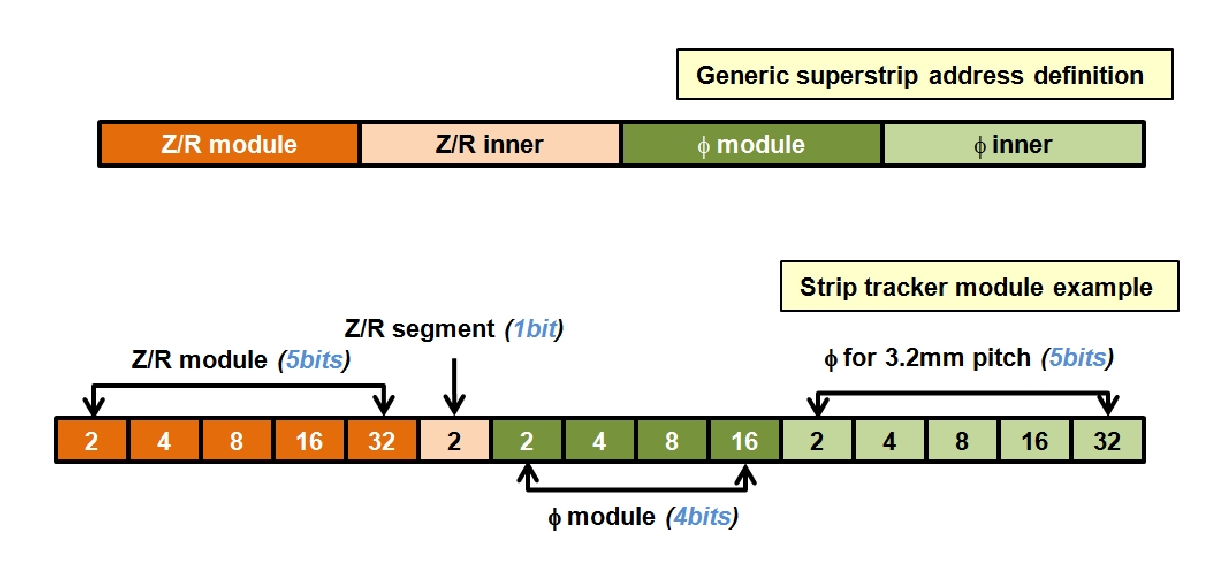
\includegraphics[width=0.6\columnwidth]{Plots/SSaddress.eps}
\caption{Address definition of a superstrip.}
\label{fig:SS_def}
\end{figure}

\noindent In order to understand the address definition, Fig.~\ref{fig:Det_to_SS} shows how a superstrip is defined in the barrel part of the tracker. Figure~\ref{fig:SS_def} shows the address definition of a superstrip. The number of bits necessary reflects the superstrip granularity and is constrained by the maximal word size acceptable by the AM chip (default is 15 bits). A first set of bits provides the module number along the corresponding coordinate: 5 bits for Z (one could have up to 24 modules in Z in one sector) and 4 for ? (up to 11 modules per sector in the outermost layer). Then, for each coordinates, a second series of bits provide the superstrip position within the module. Fig. 6 shows a tracker strip module (in green), divided into 2 segments in Z and 1024 strip in ?. Therefore in order to describe all the position, one would need only 1 bit for Z, and 10 bits for ?. In practice, a certain number of strips are grouped to form the superstrip, in our case 32, thus leading to 5 in the address. For the endcap the coding is the same, with z being replaced by r (equivalence is made between disks and layers, ladders and rings). 



\clearpage
